\section{Materials}

	All anhydrous and non-anhydrous solvents had a reagent grade purity; were purchased from Sigma-Aldrich and used without any additional treatment.
	
	\Acr{fai}, \acr{mabr} and \acr{mai} were either synthesized in-house (see page \pageref{methods-MAI}) or bought from GreatCell Solar.
	
	\PbItwo (99~\%), \PbBrtwo (99.999~\%), \CsI (99.999~\%), \PbCltwo (98~\%), anhydrous chlorobenzene, anhydrous \gls{dmf}, and anhydrous \gls{dmso} were bought form Sigma-Aldrich and kept in a nitrogen-filled glovebox.
	
	Titanium(IV) isopropoxide (97~\%), acetylacetone, and \glsdesc{litfsi} (\gls{litfsi}) were bought from Sigma-Aldrich.
	
	4-tert-butylpyridine and hydroiodic acid (57~m/m\% in water) were bought from Sigma-Aldrich and kept in a fridge (the colour of both these reagents change with ageing when kept out of the fridge).
	
	\Spiro was bought from 1-Material and stored in a nitrogen-filled glovebox.
	
	Methylamine in methanol (40~w/w\%, \SI{\approx9.8}{\Molar}) was bought from Tokyo Chemical Industry.
	
	\Tae1, \tae3, and \tae4 molecules were used as received from Inés García-Benito, Agustín Molina-Ontoria and Nazario Martín (IMDEA, Madrid). The synthesis of \tae1 has been described in \authoryear{Cabau2015a} and \authoryear{Choi2015b}. The synthesis of \tae3 and \tae4 has been described in CITATION.
	
	Patterned \gls{fto} substrates with sheet resistance of \SI{7}{\ohm\per\sq} (TEC7) on \SI{2.2}{\mm} thick and \SI{14.8x14.8}{\mm} wide Pilkington glass were bought from Xinyan Technology Ltd.
	
	Patterned \gls{ito} substrates with sheet resistance of \SI{15}{\ohm\per\sq} on \SI{1.1}{\mm} thick and \SI{15x15}{\mm} wide glass were bought from Xinyan Technology Ltd.
	
	Dust free cloths Super Polx 1200A \SI{23x23}{\cm} were bought from Berkshire.
	
	\Gls{pedotpss} Clevios P VP.AI 4083 was bought from Heraeus.
\section{Equipments}
	
	Spin coating depositions in the nitrogen-filled glovebox were performed with a SPIN150 equipment (this model does not require a gas inlet, which would be troublesome in a glovebox) from SPS Europe where the transparent cap was removed from the lid for helping solvent vapours removal. The internal side of the deposition chamber was covered with aluminium foil and this foil replaced between an user and the next. Most common failure: exhaustion of the supposedly \SI{20}{\year} lasting nonvolatile SRAM (or nvSRAM or BattRAM, a perfect example of planned obsolescence and vendor lock-in altogether).
	
	Spin coating depositions in the clean room were performed with a XXXXXXXXXXXXXXXXXXXXXXXXXXXXXXXXXXX
	
	Current-voltage scans were performed with a Tektronix Keithley 2400 with firmware revision C30 programmable digital source meter connected to a computer via a GPIB-USB-HS adapter from National Instruments, connected to the solar simulator for the shutter control via a RS-232 (Keithley side) to coaxial (solar simulator side), and connected to the device to measure via a coaxial (devices side) to 2 banana plugs (Keithley side). Even if Keithley is a remarkable piece of hardware, I observed various times sparks in my devices when connecting them to the equipment, so I warmly suggest to manually set the Keithley in current measure mode with zero applied voltage, start the measure with the devices not connected and finally connect the devices.
	
	Illumination for current-voltage scans was provided by a Sun 2000 solar simulator (\SI{150}{\W}) bought from ABET Technologies. The proper filters of the lamp were set to simulate the AM 1.5G solar spectrum. The light intensity at the measurement position was measured via the short circuit current of a small photodiode calibrated with a certified (NREL) silicon photodiode. Most common failure: lamp power supply.
	
	Background illumination for \acr{tpv}, \acr{tpc}, and \acr{ce} measurements was provided via a white light LED ring assembled in-house with LED from LUXEON Lumileds.
	
	Perturbation illumination for \acr{tpv} and \acr{tpc} measurements was provided by a nanosecond PTI GL-3300 nitrogen laser. The wavelength was selected using a dissolved molecular dye. The pulse intensity was attenuated with a semi-transparent glass for ensuring the small perturbation regime. The spark in the nitrogen laser emits a strong and unwanted electromagnetic pulse that can be received from all non-coaxial cables and from the samples holder, adding a transient noise to the oscilloscope measurement.
	
	The voltage transients for \acr{tpv}, \acr{tpc}, and \acr{ce} measurements were registered with a Yokogawa DLM2052 oscilloscope connected to the device holder via coaxial cable and to the computer via an USB2 port (the transfer speed could be better if an Ethernet connection were used).
	
	The devices holder is designed for holding 4 devices with 4 independent diodes each (the bottom contact is assumed to be in common, the top ones are isolated) and consists in an airtight container topped with a quartz window. It was designed and fabricated by Ikerlan. The holder has at least one gold tip for each diode's electrode, the contact is ensured by springs pushing the tips towards the devices. A printed circuit board connects the gold tips to a coaxial connector via two rotatory selectors which allows to select the needed diode.
	
	Thicknesses were measured furrowing layers with an hard object and measuring the elevation profile with an Ambios Tech. XP-1 profilometer.
	
	Cross sectional \acr{sem} images were acquired using a Jeol JSM-6400 microscope.
	
	Superficial \acr{esem} images were acquired at low voltage (20 keV) in a FEI Quanta 600 FEG microscope.
	
	Calcination was performed with a muffle oven XXXXXXXXXXXXXXXXXXXXXXXXXXXXXXXXXXXXXXXXXXXXXXX. Most common failure: users setting very badly the heating ramp.
	
	UV/ozone treatment was performed with a T10X10/OES ultra-violet ozone cleaning system from UVOCS. Most common failure: insufficient gas extraction flow detected by differential pressure meter on the rear, it can be partially configured via a screw.
	
	Perovskite layers annealing were performed with a highly homogeneous hotplate XXXXXXXXXXXXXXXXXXXXXXXXXXXXXXXXX
	
	Perovskite deposition was performed in a nitrogen-filled glovebox by XXXXXXXXXXXXXXXXXXXXXXXXXXXXXXXXXXXXXXXXXXX
\section{Synthesis, handling and purification}

	\subsection{\Acr{mai} synthesis}\label{methods-MAI}
	
		%Reference in laboratory notebook: [ig15, ig18, ig31, ig83].
		
		The synthetic method was inspired by \cite{Im2011a, Aharon2014, Williams2014, Etgar2012a, Nagaoka2015}.
		
		In a \SI{500}{\ml} one-necked flask (a big vessel helps later for drying) opened at air, \SI{14}{\ml} of a methylamine in methanol (40~w/w\%, \SI{\approx9.8}{\Molar}) were introduced. Dropwise, \SI{15}{\ml} of hydroiodic acid in water (57~m/m\%) was added while stirring and cooling at \SI{0}{\celsius}. This mixture was left stirring at room temperature and then still overnight covering the flask neck without completely closing it.
		The solution was evaporated in a vacuum-assisted rotatory evaporator at \SI{60}{\celsius}.
		The obtained white solid was scraped and transferred on a funnel with membrane filter (Sartorius, \gls{ptfe}). It was washed with diethyl ether and the diethyl ether discarded. The solid was dissolved with ethanol, using as little volume as possible and vacuum was used for forcing the ethanol through the filter. The solid was recrystallized pouring abundant diethyl ether, then filtered, washed with diethyl ether and dried at vacuum overnight.

	\subsection{Lead salts handling}
		
		 Lead iodide and bromide bottles have to be opened in a nitrogen-filled glovebox. The failure in keeping the lead containing precursors away from oxygen seems to cause the formation of some lead oxide, a remaining non-soluble solid in the precursors solution which would have to be filtered away.
		 
	\subsection{Dense titania precursors solution}\label{precursors_tio2}
		
		The precursor solution for the dense \TiOtwo layer was prepared using \SI{0.65}{\ml} of titanium(IV) isopropoxide and \SI{0.38}{\ml} of acetylacetone (strongly exothermic, add dropwise) in \SI{5}{\ml} of ethanol. The solution can be used just for a few days after preparation. Some hydrolysed product can be present in the solution, so it has to be filtered (\gls{ptfe}, \SI{0.2}{\um}) just before the usage. The reader should consider the more stable and commercial precursor titanium diisopropoxide bis(acetylacetonate) as a convenient alternative.
		
	\subsection{\Acr{mapicl} perovskite precursors solution}\label{precursors_mapicl}
	
		The solution was prepared in the laboratory.
		
		In a vial, \SI{400}{\mg} of \acr{mai} and \SI{230}{\mg} of \PbCltwo (98~\%) were weighted. Then \SI{1}{\ml} of anhydrous \gls{dmf} was added and the solution was stirred at \SI{65}{\celsius} for \SI{1.5}{\hour}. The solution was not filtered and was used the same day of preparation.

	\subsection{\Acr{csfamapbibr} perovskite precursors solution}\label{precursors_csfamapbibr}
		
		In a nitrogen-filled glovebox, \SI{507}{\mg} of \PbItwo, \SI{73.4}{\mg} of \PbBrtwo, \SI{172}{\mg} of \acr{fai} and \SI{22.4}{\mg} of \acr{mabr} were weighted and mixed in a \SI{5}{\ml} vial. For reducing the effect of static charging on the weighting process in the glovebox, a stainless steel weighing boat was specifically fabricated. Already at this phase some reactivity can be seen between the mixed solids (lead based perovskites are known to be possible to synthesize in a mechanosynthesis solid-solid fashion), nevertheless this mixture can be stored in the glovebox for weeks without any effect on the devices' resulting efficiency.
		
		The very day of the deposition, \SI{0.2}{\ml} of anhydrous \gls{dmso} and \SI{0.8}{\ml} of anhydrous \gls{dmf} were added to the solid mixture of precursors. The solution was vigorously stirred (a magnetic stirrer as big as the vial bottom allowed us to dissolve all the solid grains) at \gls{rt} for \SI{1}{\hour}. Heating or storing the solution for days has been observed to result in a yellow perovskite layer when deposited and annealed, so some kind of detrimental transformation is evident to happen in the solution, hindering its storage for long time. Finally \SI{42}{\ml} of
		a \SI{1.5}{\Molar} \CsI solution in \gls{dmso} were added to the previous solution. The solution was filtered (\gls{ptfe}, \SI{0.2}{\um}) just before its usage: Even if the solution looks clear it can contain solid particles.

	\subsection{\Spiro and other \acr{htm} solutions for bottom cathode cells}
	
		A solvent with additives mix was prepared adding \SI{197}{\umol} of 4-tert-butylpyridine (\SI{28.8}{\ul}) to \SI{1}{\ml} of anhydrous chlorobenzene, then \SI{32}{\umol} of \gls{litfsi} (\SI{9.1}{\mg}) were added. The presence of 4-tert-butylpyridine enables the solubility of \gls{litfsi} in chlorobenzene.
		
		\Glsdesc{spiro} (\spiro) \acr{htm} solution was prepared dissolving \SI{59.0}{\umol} of \spiro (\SI{72.3}{\mg}) in \SI{1}{\ml} of the aforementioned solvent with additives mix.

		Other \acr{htm} solutions for bottom cathode cells were prepared dissolving either \SI{29.5}{\umol} of \glsdesc{tae1} (\tae1, \SI{36.6}{\mg}), \SI{19.7}{\umol} of \glsdesc{tae3} (\tae3, \SI{24.4}{\mg}), or \SI{9.83}{\umol} of \glsdesc{tae4} (\tae4, \SI{12.1}{\mg}) in \SI{1}{\ml} of solvent with additives further diluted with chlorobenzene in a 1:1, 1:2, 1:5 ratio respectively, in order to preserve the \acr{htm} to additives molar ratio of the \spiro solution (roughly \SI{3}{\eq} of 4-tert-butylpyridine and \SI{0.5}{eq} of \gls{litfsi}). The lower concentrations were used due to the lower solubility of these \acr{htm} as compared to \spiro one.
		
		The solutions were prepared in a nitrogen-filled glovebox in order to have control over the oxygen oxidation degree of the molecules.

\section{Perovskite Solar Cells}

	The "top" or "bottom" naming refers to the cell orientation during fabrication, so the "bottom" layer is the one closer to the glass substrate.

	\subsection{Top Cathode Perovskite Solar Cells}

		\subsubsection{Anode and HTM Substrate Preparation}
			% based on ig77
			This process was performed in a class 7 clean room.
		
			\Gls{ito} coated substrates were cleaned in an ultrasound bath with acetone for \SI{15}{\min}, isopropanol for \SI{15}{\min} and rubbed with a dust-free cloth. Finally, an UV/ozone treatment was performed for \SI{20}{\min}.
			\Gls{pedotpss} was filtered on \gls{pes} membrane (\SI{0.22}{\um}) 
			and deposited via spin coating (static dispensing, \SI{110}{\ul}) with a first step where the speeds regulates the thickness of the layer and a second step for removing the residual liquid accumulated at the substrate corners. The conditions are reported in Table~\ref{pedotpss_thickness} and the thicknesses were obtained via absorbance of the film at \SI{2150}{\nm} (the absorption in the visible region is very weak) calibrated to the a very thick layer measured with the profilometer. A rough relation between the thickness $d$ and the spinning speed $f$ (with \SI{1000}{\rpm\per\s} acceleration) was found as $d = \frac{1820}{\sqrt{f}}$. Substrates were dried at \SI{110}{\celsius} for \SI{20}{\min} and stored in a nitrogen-filled glovebox for avoiding moisture absorption.
			
			\begin{table}%[h]
				\caption{\Gls{pedotpss} deposition conditions and resulting thickness}\label{pedotpss_thickness}
				\begin{center}
					\begin{tabular}{c c c | c c c | c}
						\multicolumn{3}{c|}{\nth{1} step} & \multicolumn{3}{c|}{\nth{2} step} & \multirow{2}{*}{thickness} \\
						acceleration & speed & time & acceleration & speed & time & \\
						\si{\rpm\per\s} & \si{\rpm} &  \si{\s} & \si{\rpm\per\s} &  \si{\rpm} & \si{\s}  & \si{\nm} \\
						\hline
						\rule[0ex]{-4pt}{3ex}
						1000&1000&60&2000&2000&3&65\\
						1000&1600&60&2000&2000&3&45\\
						1000&4500&30&500&3500&30&27\\
					\end{tabular}
				\end{center}
			\end{table}

		\subsubsection{\Acr{mapicl} Perovskite One Step Fabrication}
			% ig71
			The deposition process was performed in a nitrogen-filled glovebox.
			
			The precursors solution (see page~\pageref{precursors_mapicl}) was deposited via spin coating (\SI{80}{\ul}, static dispensing, loading time \SI{5}{\s}) with an acceleration of \SI{1000}{\rpm\per\s}, a speed of \SI{1900}{\s} for \SI{40}{\s}. The substrate was moved directly to a hotplate at \SI{100}{\celsius} and annealed for \SI{80}{\min}, resulting in a \SI{430}{\nm} thick perovskite layer. The film is colourless just after deposition, then it turns to brown, yellow and finally black on the hotplate.
		
		\subsubsection{\Acr{mapi} Perovskite Two Step Fabrication}
			% based on ig79
			This process was performed in a nitrogen-filled glovebox
			while constantly purging with a nitrogen flow for reducing the \gls{dmf} and \gls{dmso} vapours concentration.
			
			\SI{460}{\mg} of \PbItwo were dissolved in \SI{1}{\ml} of a 23:2~v/v blend of anhydrous \gls{dmf} and anhydrous \gls{dmso}. This solution was stirred at \SI{50}{\celsius} for \SI{1}{\hour}. \SI{50}{\mg} of \acr{mai} were dissolved in \SI{1}{\ml} of a 3:1~v/v blend of anhydrous isopropanol and ethanol. A \PbItwo layer was deposited from the unfiltered solution via spin coating (static dispensing, \SI{80}{\ul}, loading time \SI{5}{\s}) with accelerations and speeds reported in Table~\ref{mapi_thickness}. After \SI{60}{\s} from the start of the spin coating, the \acr{mai} solution (\SI{100}{\ul}) was dynamically dispensed on the centre of the spinning substrate with a \SI{100}{\ul} micropipette keeping it tilted and depositing an uninterrupted stream. The substrate was then moved directly from the spin coater to an hotplate at \SI{100}{\celsius} and annealed for \SI{15}{\min}. The thicknesses reported in Table~\ref{mapi_thickness} were measured using the profilometer. 
			
			\begin{table}%[h]
				\caption{\Acr{mapi} deposition conditions and resulting thickness}\label{mapi_thickness}
				\begin{center}
					\begin{tabular}{c c c | c}
						acceleration & speed & time & thickness \\
						\si{\rpm\per\s} & \si{\rpm} &  \si{\s} & \si{\nm} \\
						\hline
						\rule[0ex]{-4pt}{3ex}
						2000&2000&90&360\\
						4000&4000&90&250\\
						8000&7500&90&180\\
					\end{tabular}
				\end{center}
			\end{table}
			
		\subsubsection{\Gls{etm} and Cathode Deposition}
			% based on ig75
			The solution was prepared in the clean room (weighting fullerene derivatives in a glovebox would be difficult due to electrostatic phenomena) and the deposition process was performed in a nitrogen-filled glovebox.
					
			\SI{30}{\mg} of \acr{pcbm70} were dissolved in \SI{1}{\ml} of anhydrous chlorobenzene and stirred at \gls{rt} for \SI{1}{\hour}. This solution was filtered (\gls{ptfe}, \SI{0.2}{\um}) and deposited in a nitrogen-filled glovebox via spin coating (static dispensing, \SI{80}{\ul}, loading time \SI{5}{\s}) with accelerations and speeds reported in Table~\ref{pcbm_thickness}. The thickness was estimated by absorbance at \SI{378}{\nm} calibrating the highest point with a profilometer measurement. A rough relation between the thickness $d$ and the spin speed $f$ was found as $d = \frac{3930}{\sqrt{f}}$ when a concentration of \SI{30}{\mg\per\ml} in chlorobenzene was used.
			
			\Gls{ito} contact was cleaned on two edges using swabs slightly wet with chlorobenzene and then \gls{dmso} (the solvent vapours can damage the perovskite layer, that's why this process is done after \gls{htm} deposition).
		
			\begin{table}%[h]
				\caption{\Acr{pcbm70} deposition conditions and resulting thickness, with a concentration of \SI{30}{\mg\per\ml}}\label{pcbm_thickness}
				\begin{center}
					\begin{tabular}{c c c | c}
						acceleration & speed & time & thickness \\
						\si{\rpm\per\s} & \si{\rpm} &  \si{\s} & \si{\nm} \\
						\hline
						\rule[0ex]{-4pt}{3ex}
						1100&1100&80&120\\
						2000&2000&60&90\\
						4000&4000&40&60\\
						8000&7500&20&40\\
					\end{tabular}
				\end{center}
			\end{table}
		
			Finally, \SI{120}{\nm} of silver were deposited by thermal evaporation in high vacuum (\SI{1E-9}{\bar}). This resulted in four independent \SI{0.09}{\cm\squared} diodes for each substrate.

	\subsection{Bottom Cathode Perovskite Solar Cells}

		\subsubsection{Cathode and \gls{etm} substrate preparation}
			This process was performed in a class 7 clean room.
		
			Pre-patterned \SI{1.5 x 1.5}{\cm} \gls{fto} coated glasses were employed as substrate. An identification code was scratched on the glass side with a diamond tip pencil. The glass dust was removed with adhesive tape and rubbing with a dust free cloth. The substrates were cleaned with ultrasonication in water with Hellmanex soap, then in deionized water, and finally in isopropanol; dried rubbing with a dust free cloth and the organic residuals were removed with an UV/ozone treatment for \SI{20}{\min}.
			
			Dense (as opposed to mesoporous) \TiOtwo layer was deposited (static dispensing, \SI{80}{\ul}) from the solution described in page~\pageref{precursors_tio2} by spin-coating at \SI{3000}{\rpm}, \SI{3000}{\rpm\per\s}, for \SI{60}{\s} (\SI{\approx 30}{\nm}) over the previously cleaned \gls{fto}. Then
			the substrates were sintered at \SI{500}{\celsius} for \SI{30}{\minute} and subsequently immersed in a \SI{40}{\milli\Molar}
			\ch{TiCl4} solution in 9~\% \ch{HCl} at \SI{70}{\celsius} for \SI{20}{\min} (this process erode the titania layer, so it's important to not exceed in the duration), cleaned with water, with isopropanol and	calcined at \SI{500}{\celsius} for \SI{30}{\min}.
			
 			The usage of a thicker glass as compared to the one used for top cathode cells and the usage of \gls{fto} in place of \gls{ito} (\gls{fto} absorbs more in the infrared region and is way rougher) are needed for resisting the high temperature processing of the titania layers.
 			
		%\subsubsection{\Acr{mapi} Perovskite Two Step Fabrication}	
			% ig87
			
		\subsubsection{\Acr{csfamapbibr} Perovskite One Step Fabrication}
		
			This process was performed in a nitrogen-filled glovebox
			while constantly purging with a nitrogen flow for reducing the \gls{dmf} and \gls{dmso} vapours concentration.
			
			Perovskite precursor solution (see page~\pageref{precursors_csfamapbibr}) was filtered (\SI{0.2}{\um}, \gls{ptfe})
			and deposited by spin-coating (\SI{80}{\ul}, static dispensing, first step \SI{1000}{\rpm}, \SI{1000}{\rpm\per\s}, \SI{10}{\s};
			second step \SI{6000}{\rpm}, \SI{1000}{\rpm\per\s}, \SI{20}{\s}; fast crystallization was induced dynamically
			dispensing \SI{50}{\ul} of chlorobenzene on the spinning substrate \SI{5}{\s} before the end of the second
			step) obtaining a \SI{500}{\nm} thick perovskite layer.
			
			The substrates were immediately transferred from
			the spin coater to a hot plate and annealed at \SI{100}{\celsius} for \SI{60}{\minute}. 
	
			After removing from the hotplate, the devices were stored in a glass Petri dish for protecting from dust deposition. It was left partially open to avoid accumulation of vapours from solvent residuals.
			 
		\subsubsection{\Acr{htm} and Cathode Deposition}
		
			The \acr{htm} solutions (\spiro, \tae1, \tae3, or \tae4) were filtered (\SI{0.2}{\um}, \gls{ptfe}) just before usage and deposited by spin-coating in a nitrogen-filled glovebox
			onto the perovskite layer (\SI{60}{\ul}, static dispensing, \spiro at \SI{4000}{\rpm}, \SI{4000}{\rpm\per\s},
			for \SI{30}{\s}; \tae1 and \tae3 at \SI{2000}{\rpm}, \SI{2000}{\rpm\per\s}, for \SI{30}{\s}; \tae4 at \SI{1000}{\rpm}, \SI{2000}{\rpm\per\s},
			for \SI{45}{\s}) and similar \acr{htm} thicknesses were obtained (\SI{\approx 100}{\nm}).
			
			\Gls{fto} contact was cleaned on two edges mechanically removing the \gls{htm} and perovskite with a needle and then using swabs slightly wet with \gls{dmso} (the solvent vapours can damage the perovskite layer, that's why this process is done after \gls{htm} deposition and just for what's remaining after mechanical scratching most of the material).
			
			Unless otherwise specified, in order to increase the
			oxidative doping of the \acr{htm} in a more or less controlled way, the devices were kept \SI{1}{\hour} in dark in a dry air chamber.
			
			Finally, \SI{80}{\nm} of gold was deposited by thermal evaporation in an ultra-high vacuum chamber
			(\SI{1e-9}{\bar}, MBraun) using a shadow mask leading to 4 diodes for substrate each with an active area of
			\SI{9}{\mm\squared}.

	\subsection{Handling and Preservation}
		In case of bottom cathode cells, the oxidation of the HTM has been proven to improve the PCE. The oxidation can be induced via a dopant, for example FK209 CITATION, or via oxygen exposure. The latter has to be performed in dark as a synergic light and oxygen contribution on the perovskite layer degradation has been reported CITATION. The oxygen can enter in direct contact with the perovskite layer due to permeability of the HTM; additionally, when a mesoporous ETM is used (e.g. titania) oxygen can diffuse rapidly through the partially infiltrated mesoporous structure. For this reason a cabinet has been modified adding of a constant dry air inlet and physically reducing the leaks of the opening door edges.
				
		\begin{figure}%[!hbtp]%
			\centering
			\begin{subfigure}[b]{0.45\textwidth}
				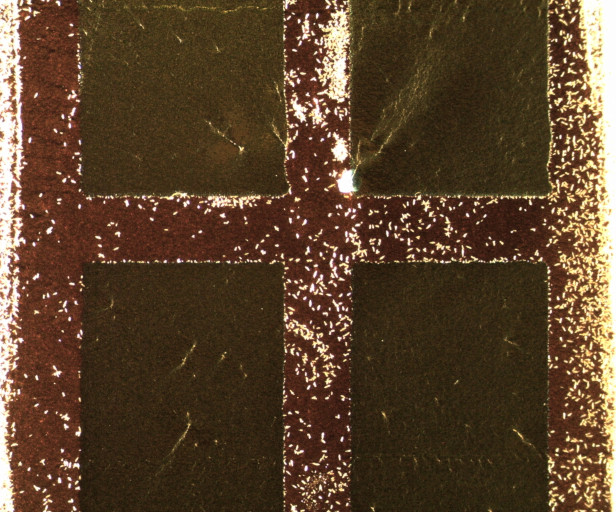
\includegraphics[width=1\textwidth]{microscope_degradation/ig93-1387-1-rescaled.jpg}
				\subcaption{Original cell, gold side.}\label{fig:microscope_degradation-start}
			\end{subfigure}
			\qquad
			\begin{subfigure}[b]{0.45\textwidth}
				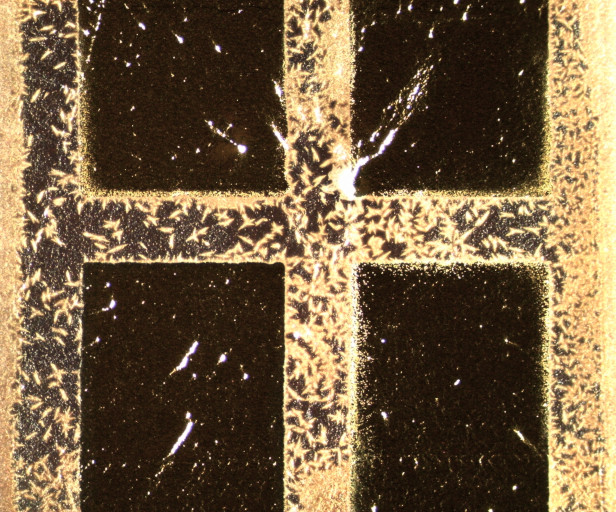
\includegraphics[width=1\textwidth]{microscope_degradation/ig93-1387-8-rescaled.jpg}
				\subcaption{After \SI{10}{\minute}, gold side.}\label{fig:microscope_degradation-end_front}
			\end{subfigure}
			\bigskip
			
			\begin{subfigure}[b]{0.45\textwidth}
				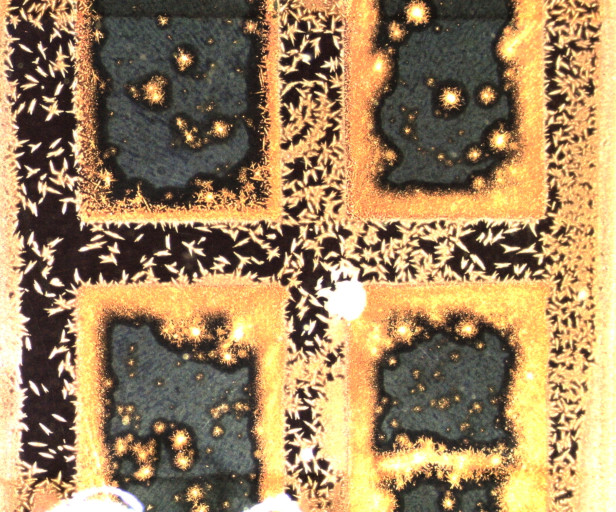
\includegraphics[width=1\textwidth]{microscope_degradation/ig93-1387-back-rescaled.jpg}
				\subcaption{After \SI{10}{\minute}, glass side.}\label{fig:microscope_degradation-end_back}
			\end{subfigure}
			\caption{Degradation of a \gls{fto}/\dTiOtwo/\mpTiOtwo/\acr{csfamapbibr}/\spiro/Au device upon \SI{10}{\minute} illumination in air.}\label{fig:microscope_degradation}
		\end{figure}
	
		In Fig.~\ref{fig:microscope_degradation} the degradation of a complete device exposed to continuous illumination for 10 minutes and ambient air conditions is shown. An analogous device kept in air but without illumination did not show any degradation as observable via optical microscopy. The gold contact was not enough for protecting the perovskite layer from degradation, as oxygen could penetrate through the mesoporous titania. Interestingly the degradation is more prominent at metallic contacts' edges, one could speculate the reason being the electrical field being higher at smaller curvature metallic edges (seems that there's no therm in English for this, in Italian is referred as "effetto punta" and corona effect concentration ad edges derives from this). It could also be that the ionic profile of perovskite when holes quasi Fermi level is pinned at gold workfunction makes perovskite more sensible to degradation, and this is more evident at edges due to oxygen diffusion being blocked by the gold layer.

		Even if storage in dark and dry air should not be damaging for perovskite solar cells, the most usual long-term storage happens in a nitrogen-filled glovebox.

\section{Solar Cells Characterization}

	All the characterization on complete devices was performed keeping them in a air tight holder filled with nitrogen. The electrical connection from the cell electrode to the external end of the holder was obtained via gold tips connected via a printed circuit board to a coaxial cable.

	\subsection{Current-Voltage Curve}

		The illumination intensity was calibrated to \SI{1000}{\W\per\square\m} (AM1.5G).
		
		The noise often observed in current-voltage scans at high sweep speeds is mainly caused by oscillations in the solar simulator illumination intensity, as an example see REFERENCE FIGURE.
		
		In literature one can easily find current-voltage curves with discontinuities, some even lucubrate about the origin of these in perovskite solar cells. Indeed this is just caused by the auto-scale feature of the Keithley equipment, disabling this the discontinuities disappears.
		
	\subsection{Charge Extraction}

		Most of the observed short-times noise (\SI{< 5E-7}{\s}) is related to the opening and closing of the transistors included in the in-house built equipment.
	\subsection{Transient PhotoVoltage}
	
		1 Hz
		
		Most of the observed noise 
	

	
	\subsection{Transient PhotoCurrent}
	
	\subsection{Differential Capacitance}
	
\section{Data Analysis and Handling}



